\subsection{Allgemeiner Aufbau}

Hier die allgemeine Struktur...

\subsection{Im Detail: Konvergenz des Metropolis Algorithmus}

Hier der Metropolis Block eines Monte Carlo Schritts mit Konvergenzverhalten

2D

\begin{figure}[H]
	\centering
	\subfigure[zufällige Startkonfiguration]{
		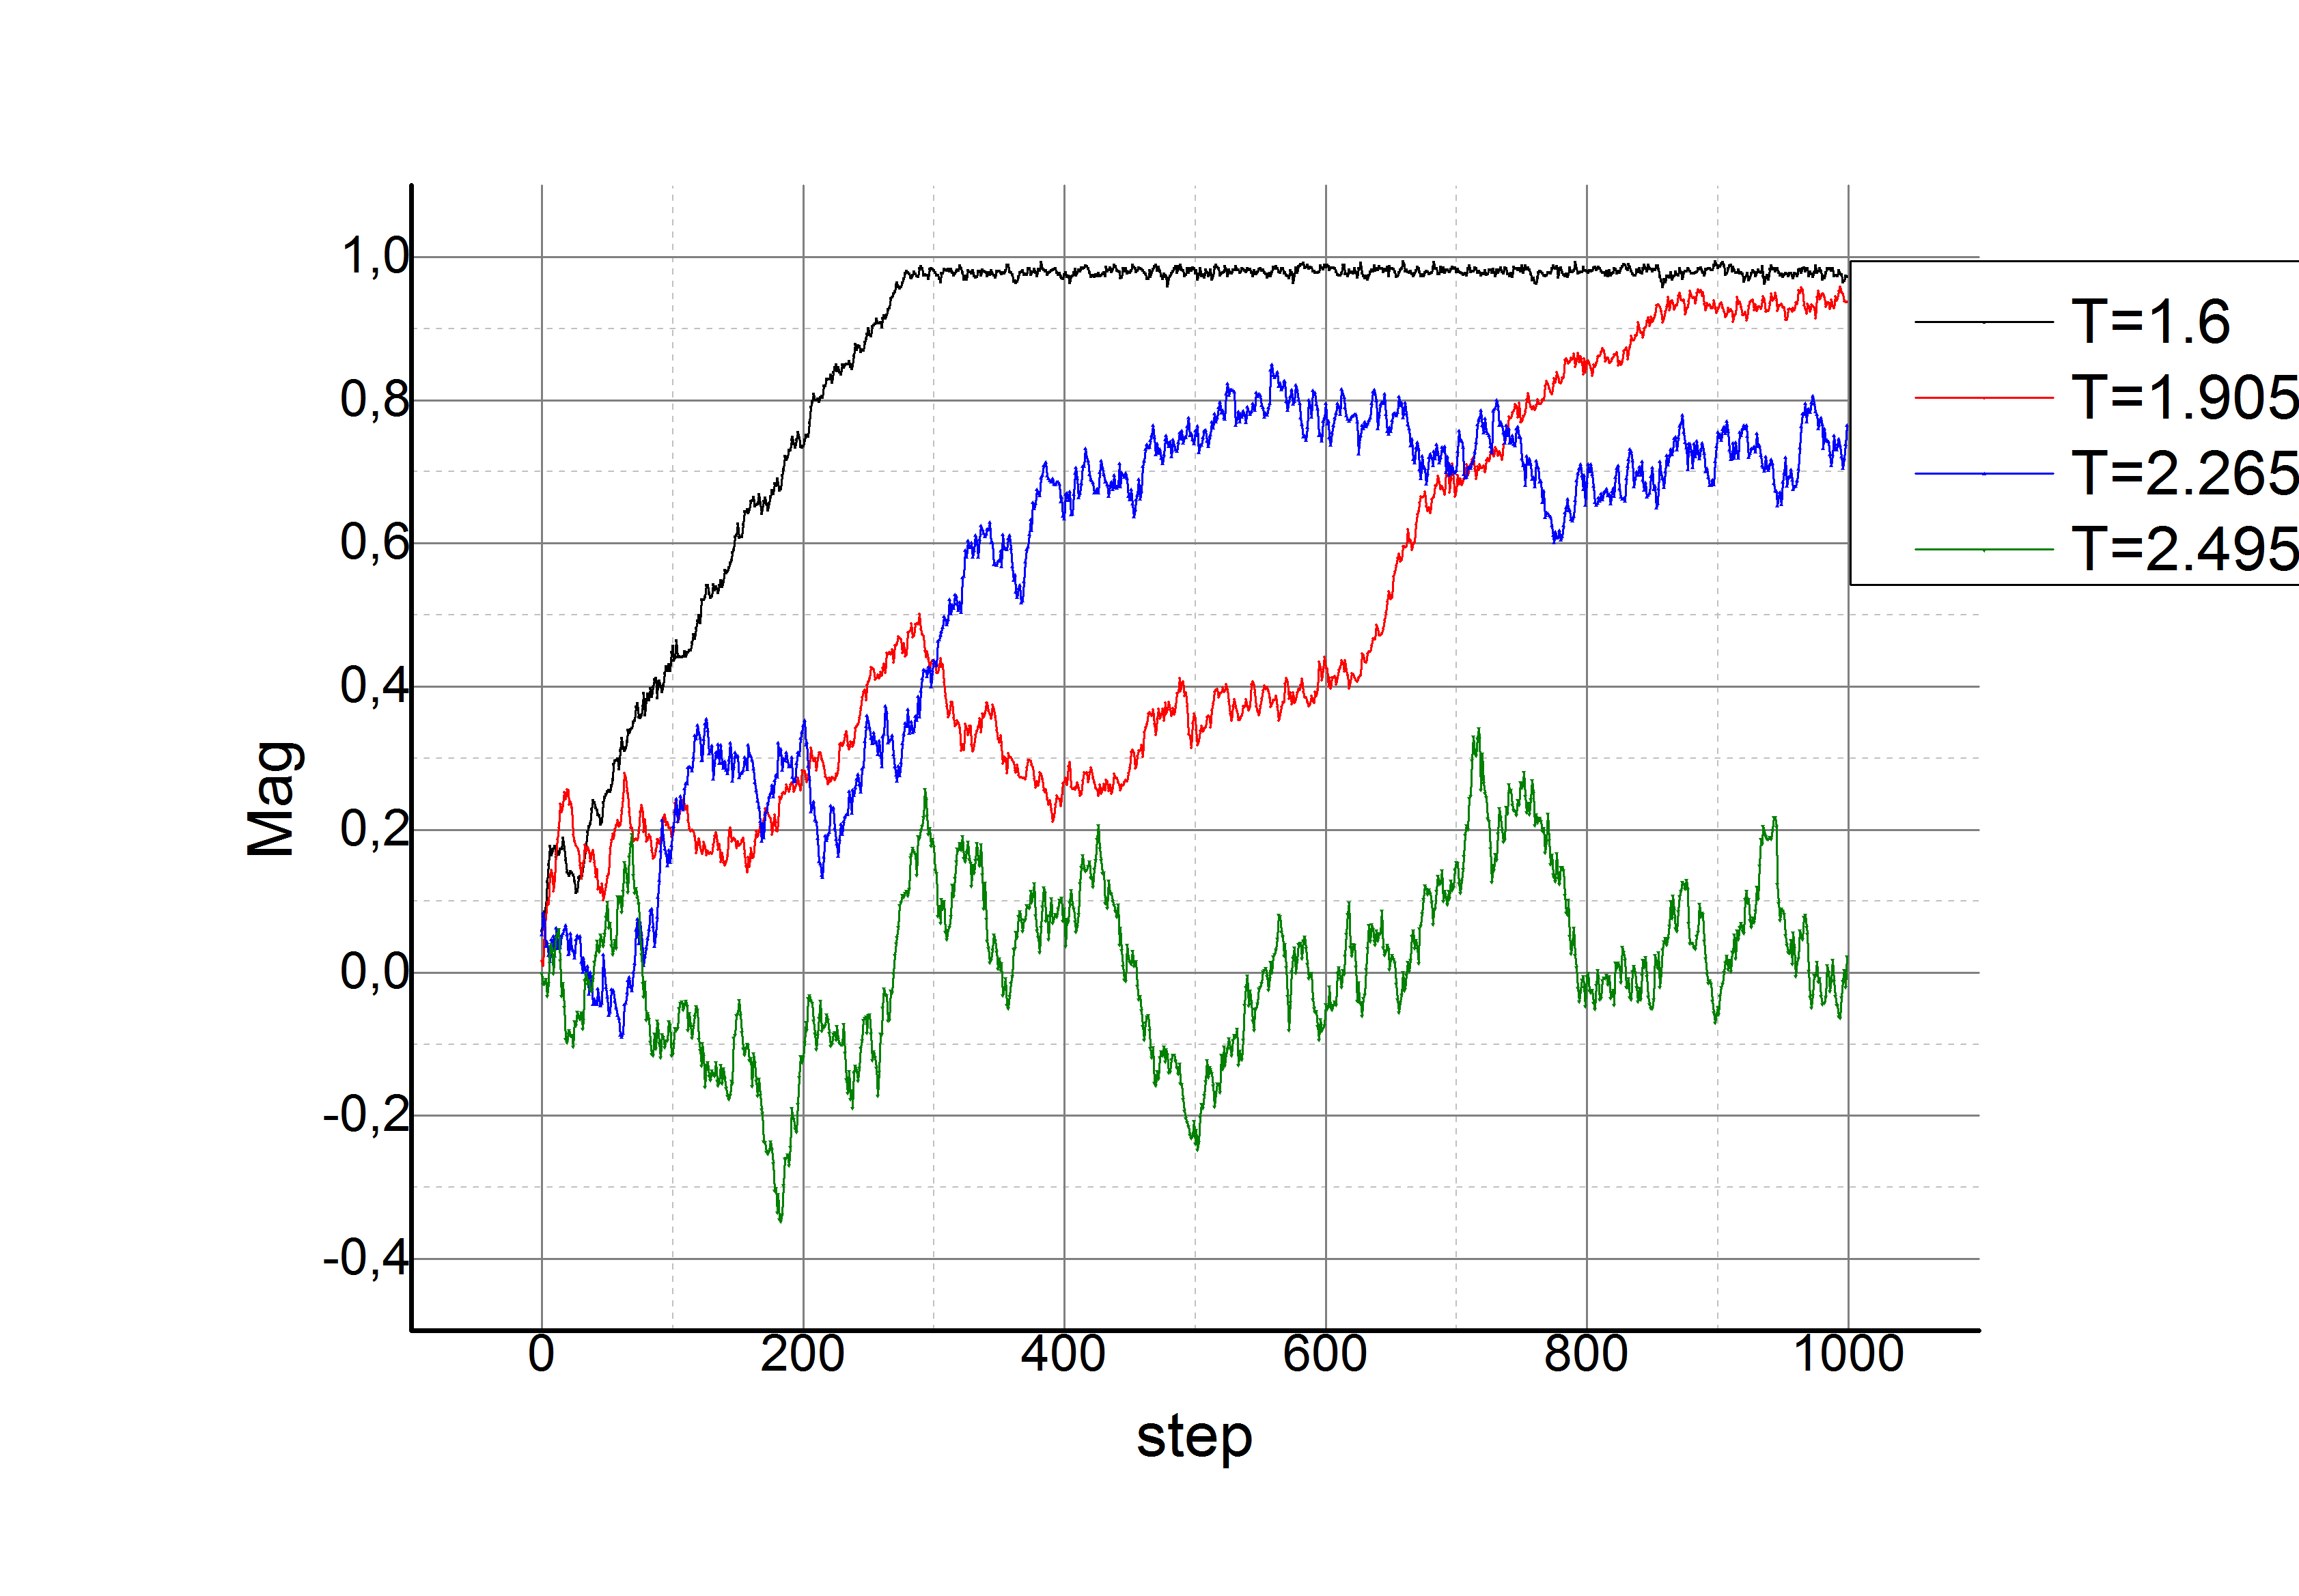
\includegraphics[width=0.47\textwidth]{../Graph_Export/MP2D/m(Steps)_r.jpg}
}	
	\subfigure[positv parallele Startkonfiguration]{
		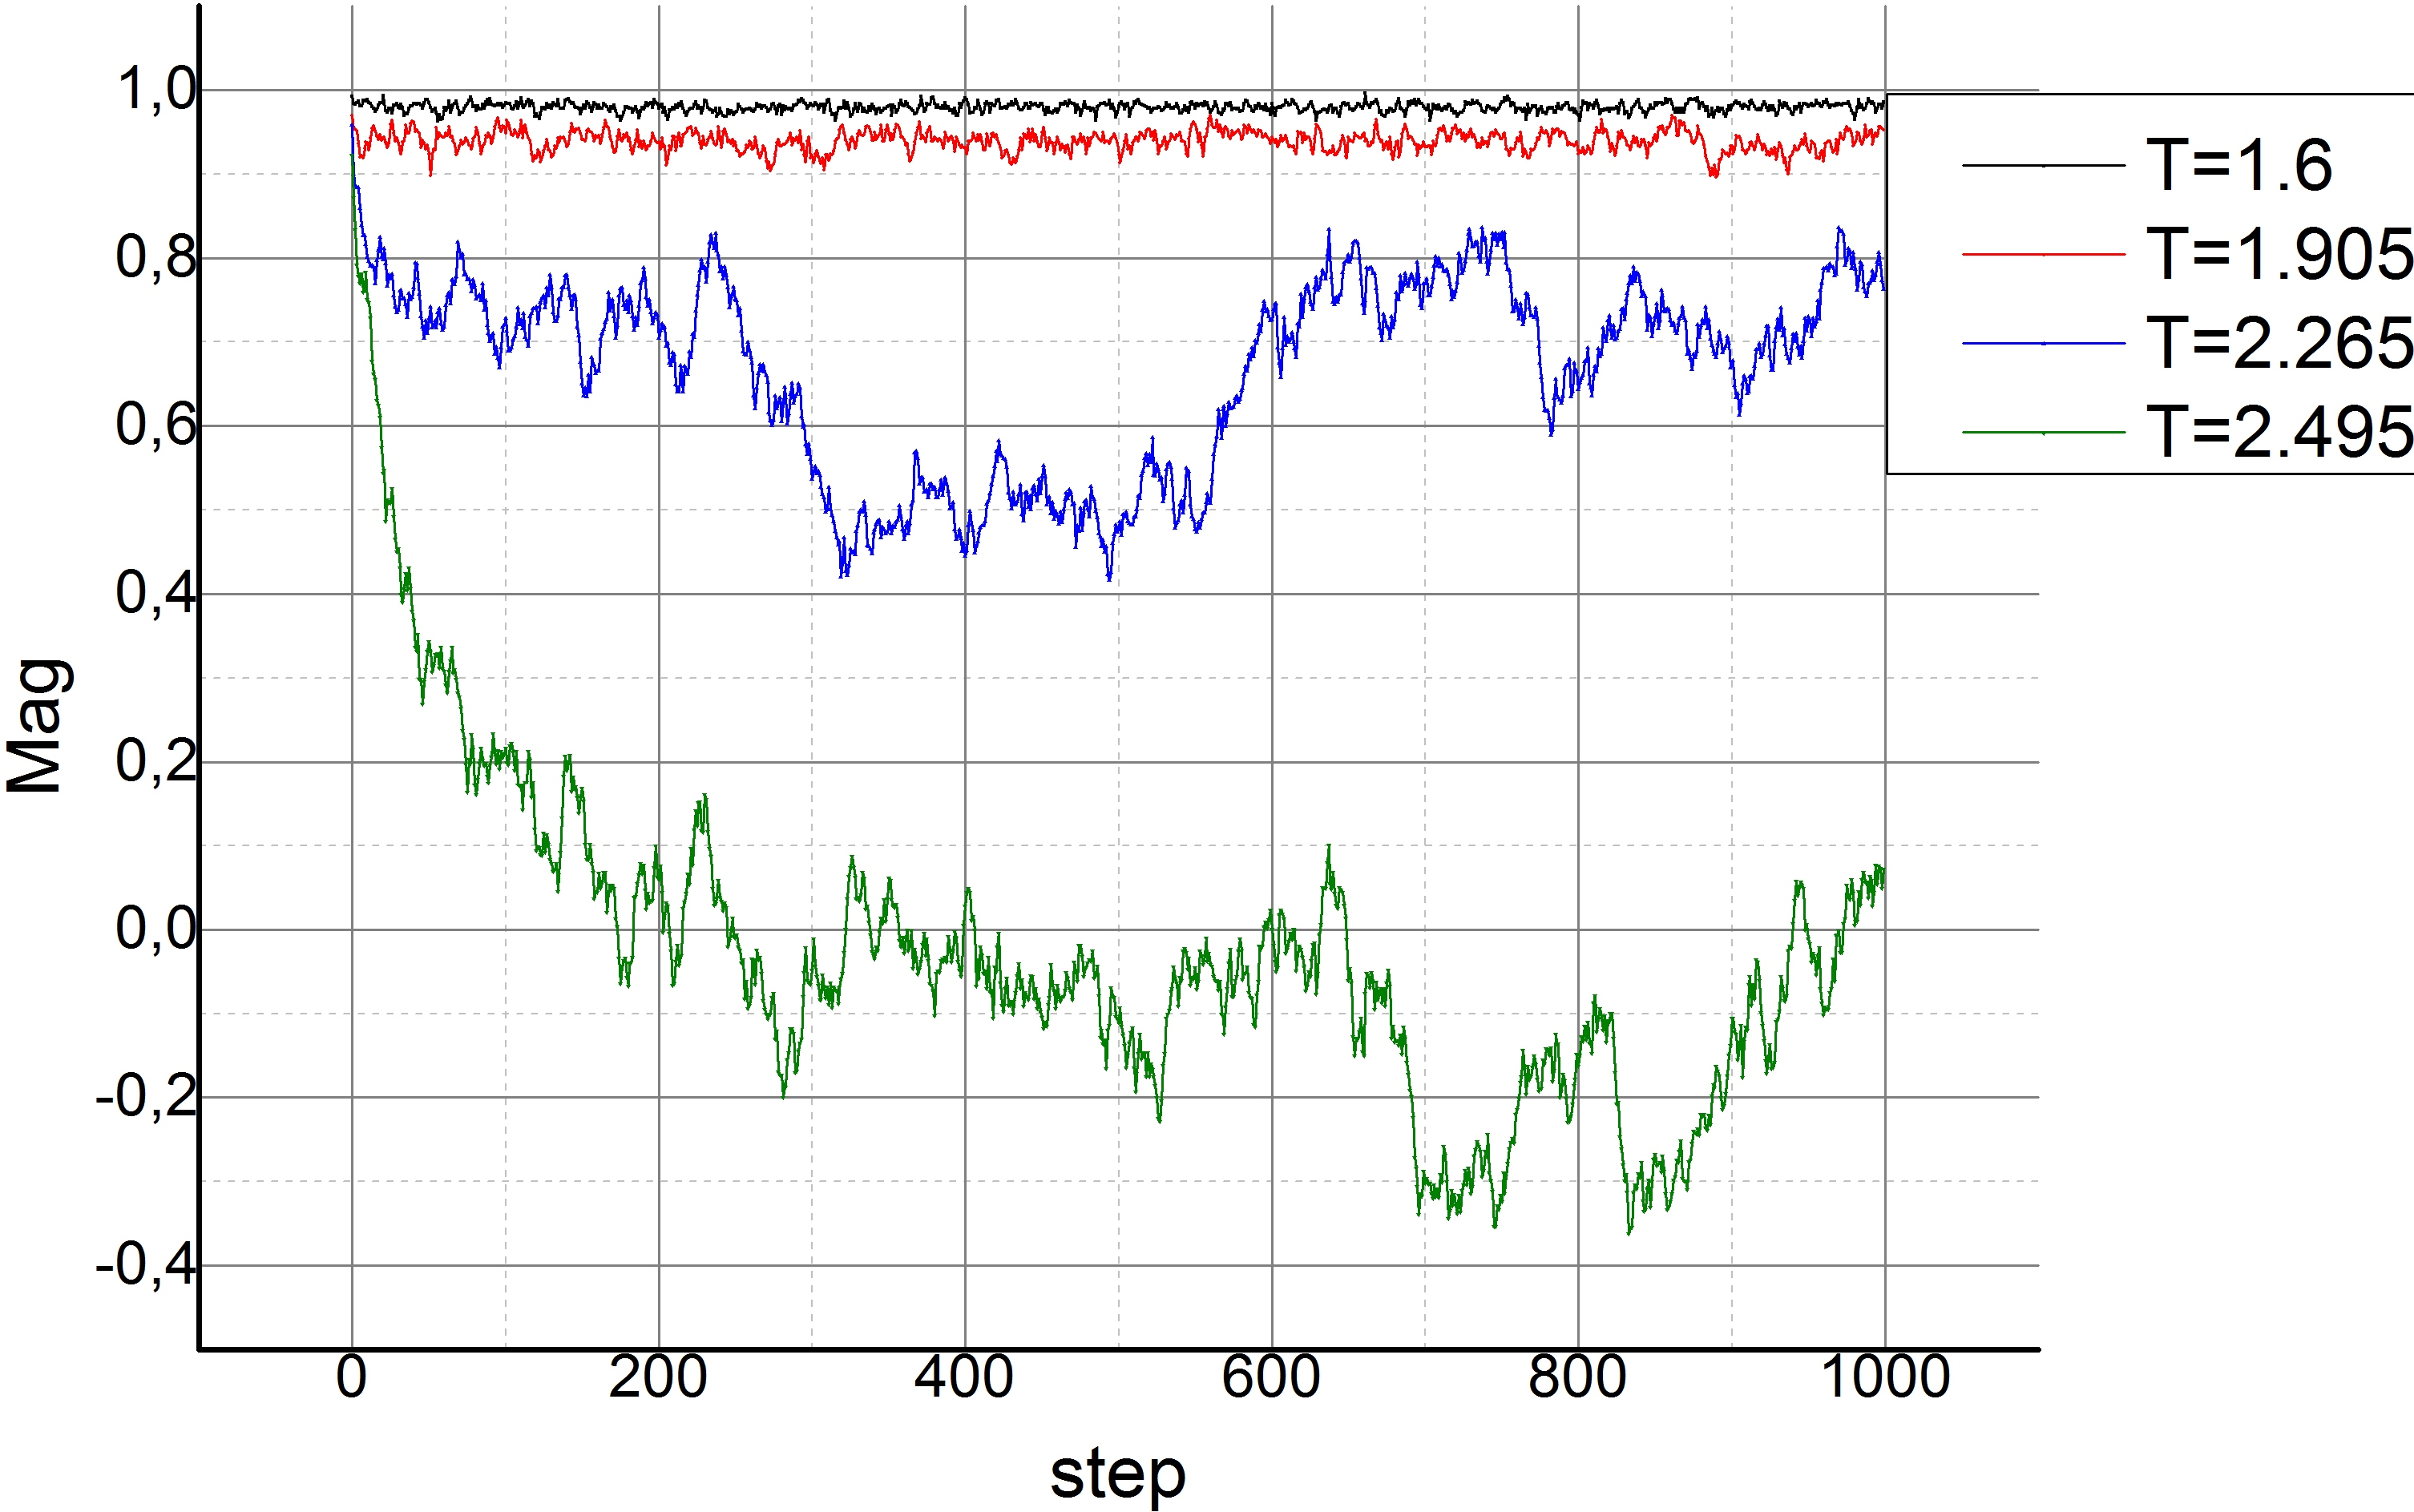
\includegraphics[width=0.47\textwidth]{../Graph_Export/MP2D/m(Steps)_p.jpg}
}		
	\caption{Konvergenzverhalten der Magnetisierung im Metropolisalgorithmus für ein zweidimensionales Gitter}
	\label{mp2dkonv}
\end{figure}

3D

\begin{figure}[H]
	\centering
	\subfigure[zufällige Startkonfiguration]{
		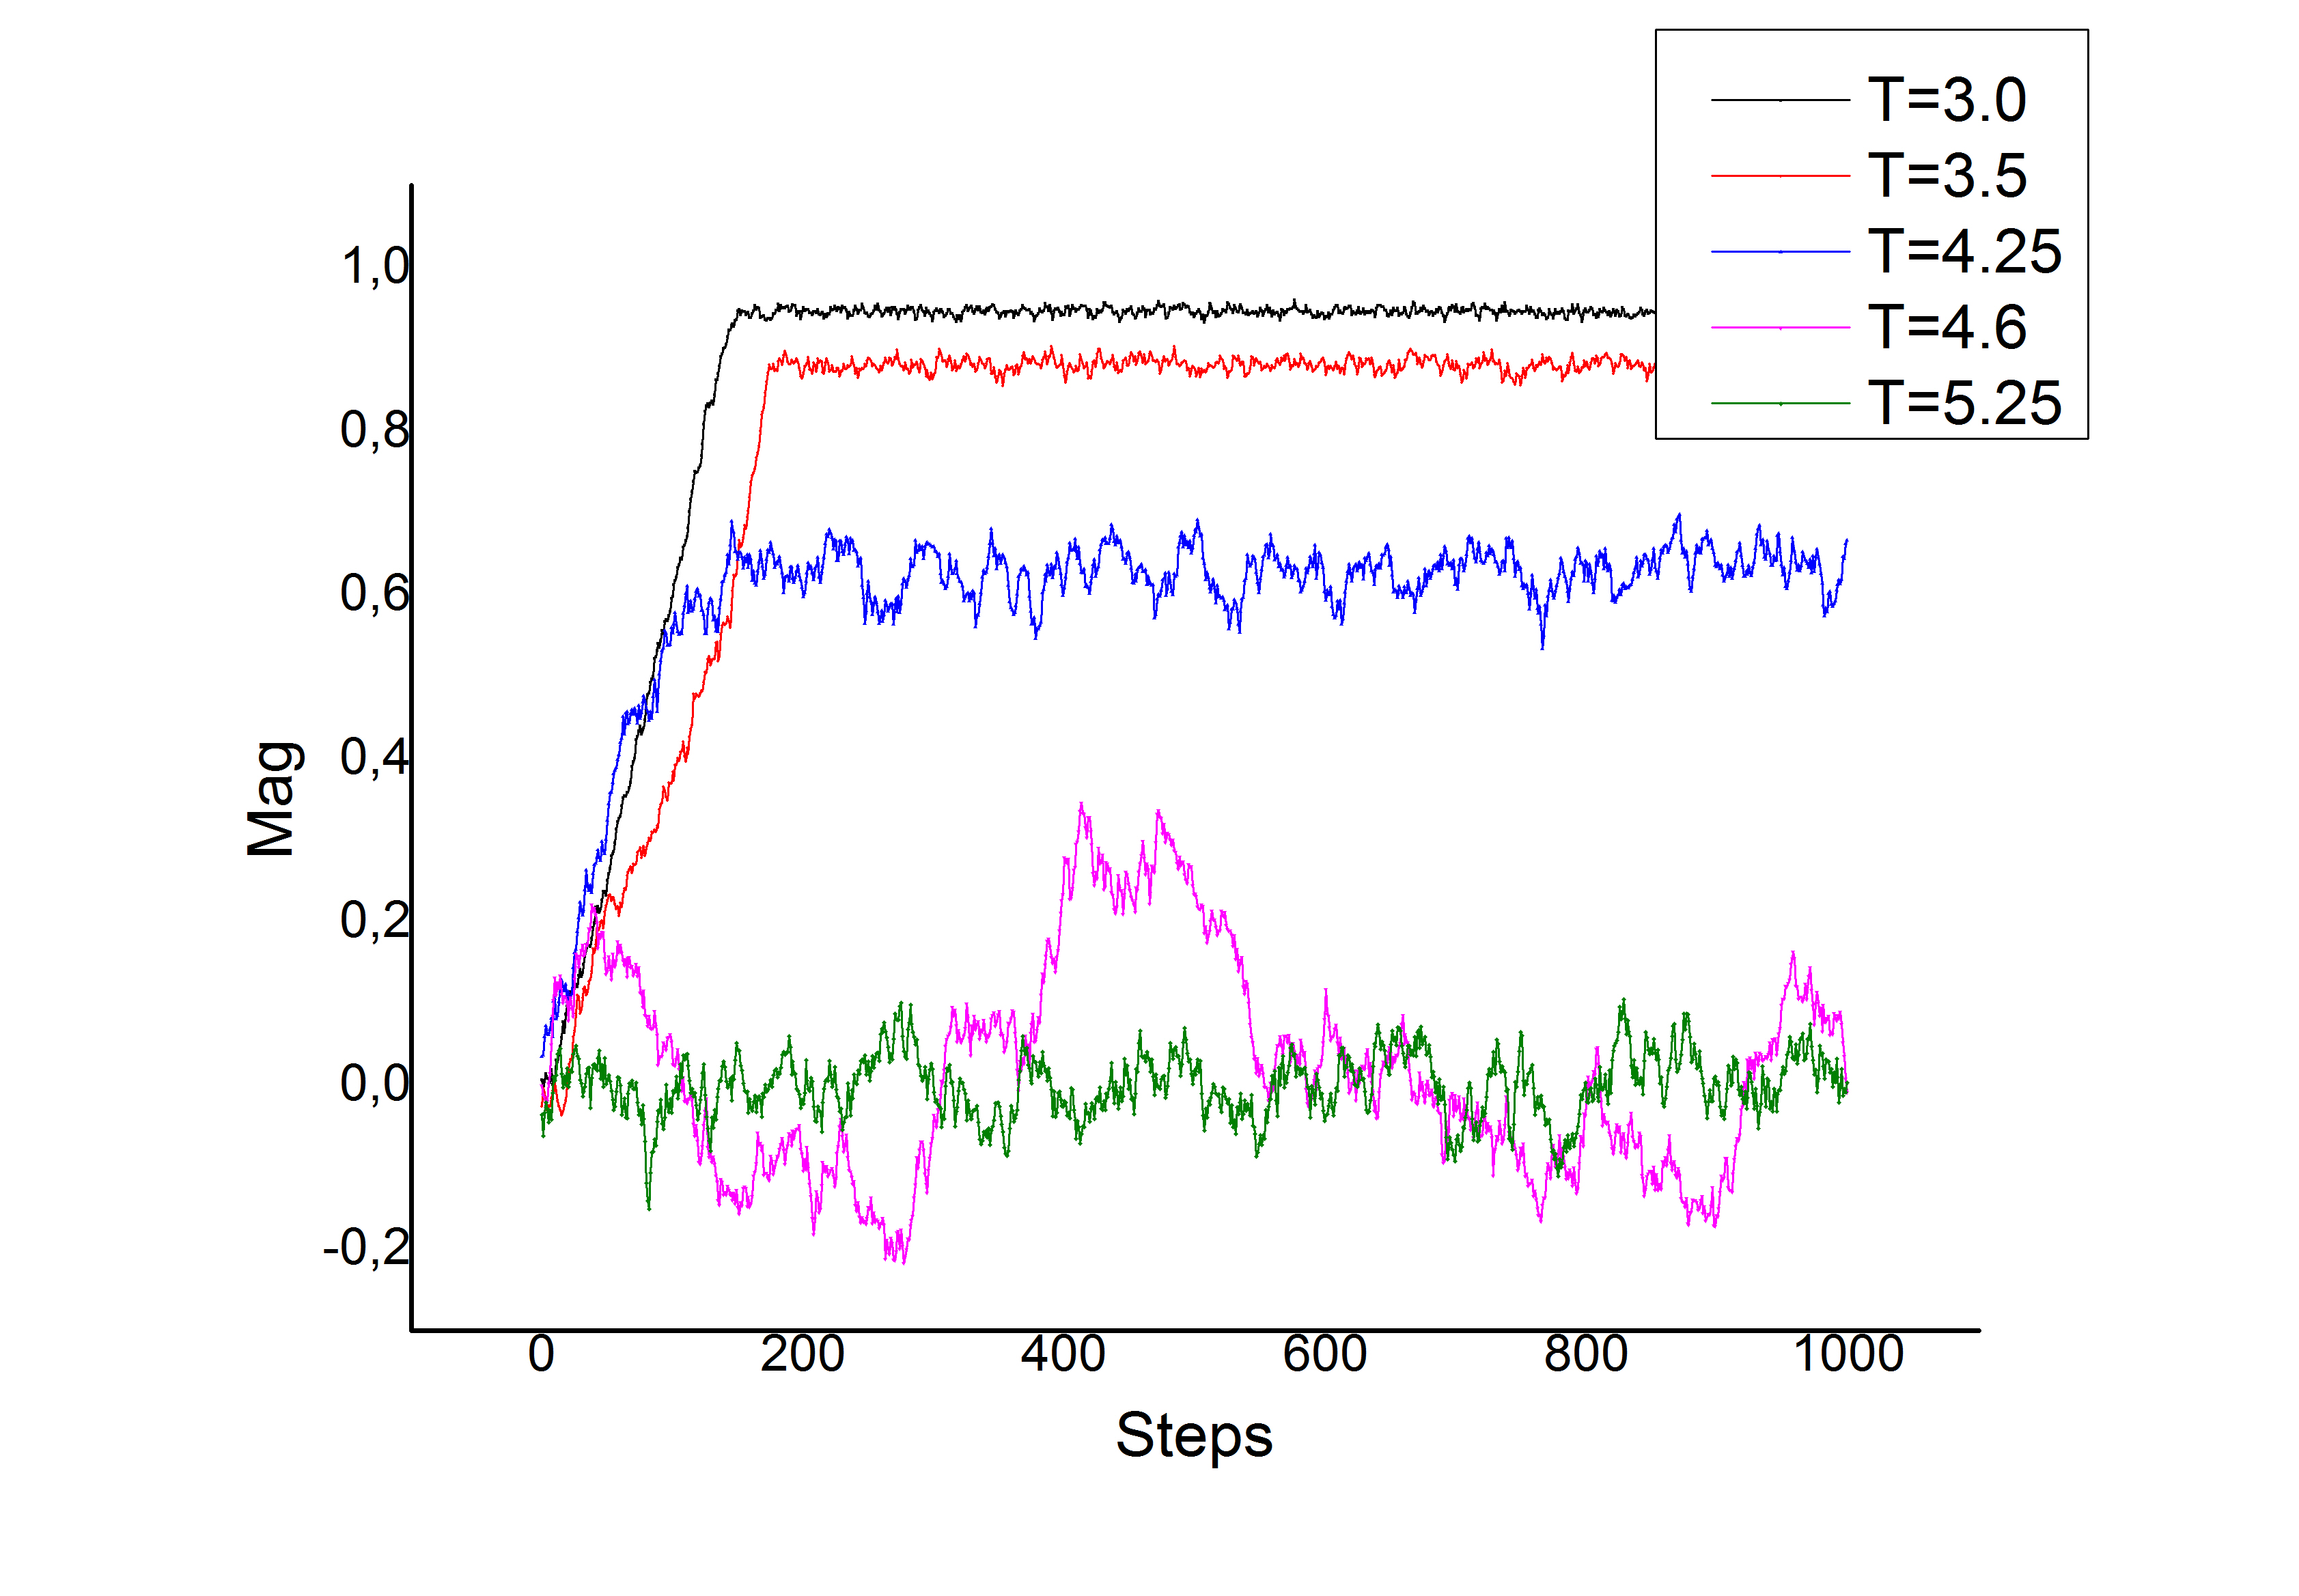
\includegraphics[width=0.47\textwidth]{../Graph_Export/MP3D/m(Steps)_r.jpg}
}	
	\subfigure[positv parallele Startkonfiguration]{
		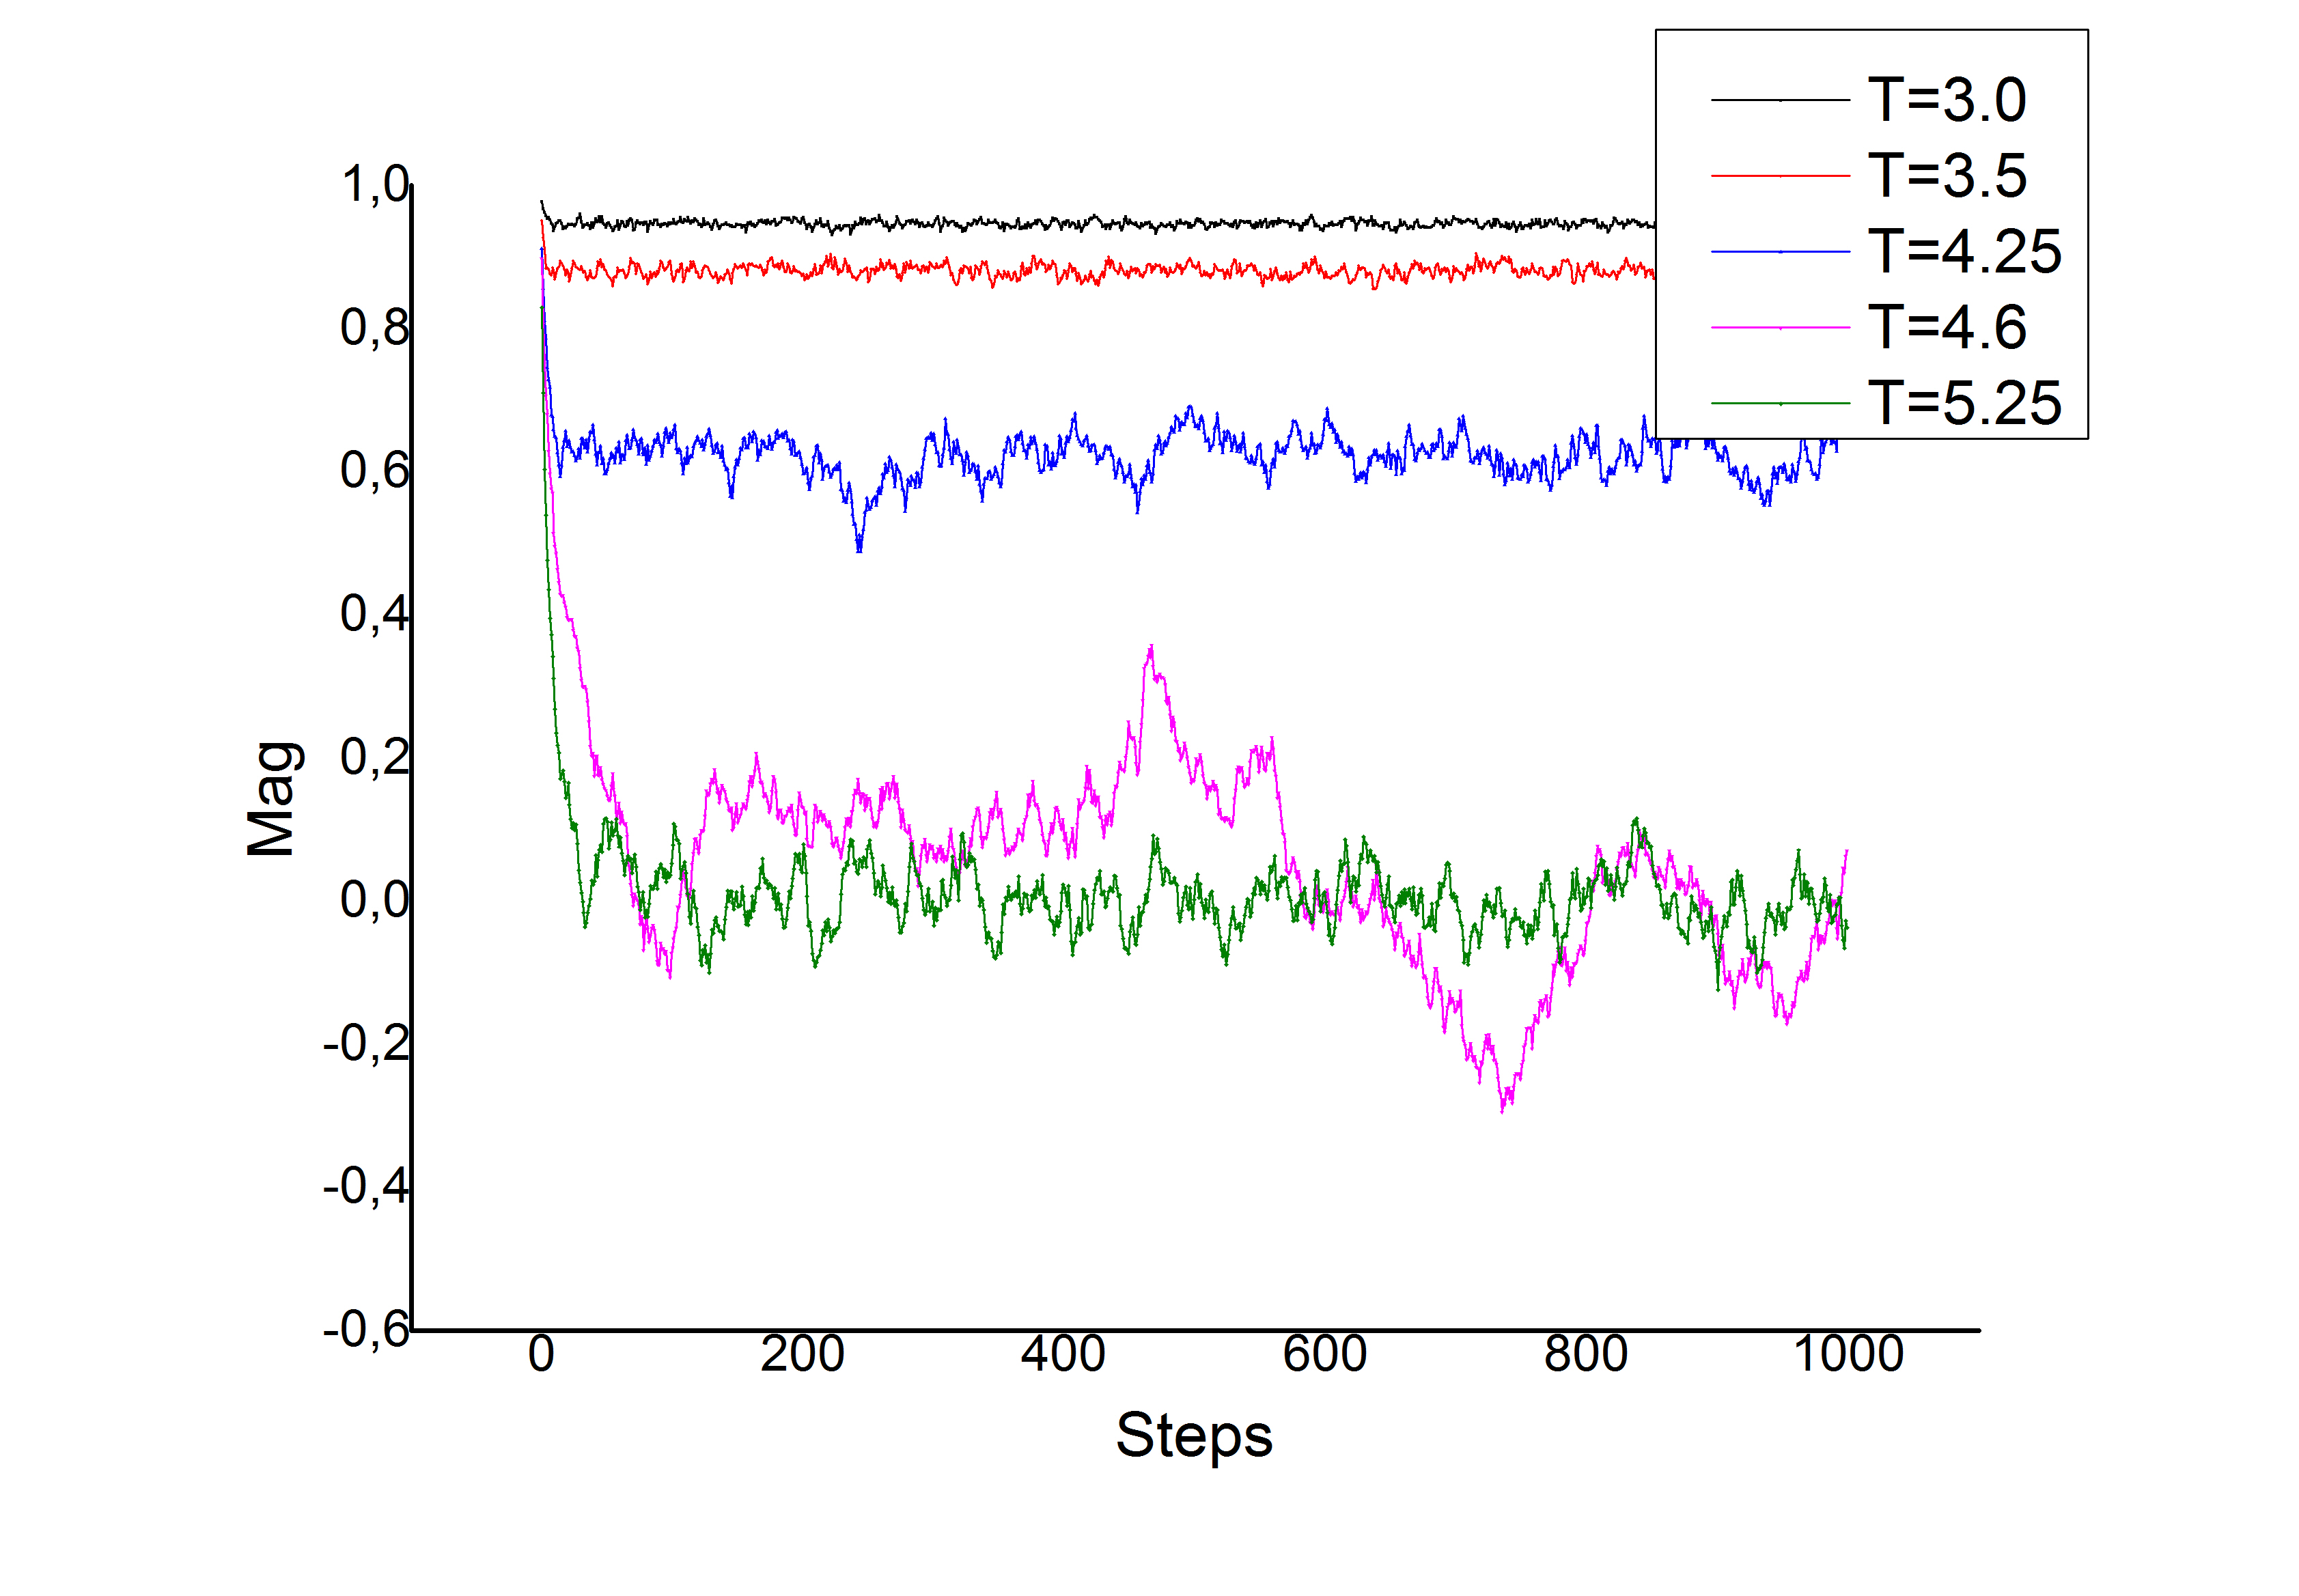
\includegraphics[width=0.47\textwidth]{../Graph_Export/MP3D/m(Steps)_p.jpg}
}		
	\caption{Konvergenzverhalten der Magnetisierung im Metropolisalgorithmus für ein dreidimensionales Gitter}
	\label{mp3dkonv}
\end{figure}

\subsection{Im Detail: Funktion weiterer Parameter}

Unterschied B T Mode etc. ..